%!TEX root = OptimalOffline.tex
%input{Siddhartha}

\begin{algorithm}
%\algsetup{linenosize=\tiny}
%\alglinenumber{linenosize=\scriptsize}
\caption{Procedure to find initial feasible policy to Problem 1 for Algorithm 2}

\footnotesize%\scriptsize
\label{init_policy}
\begin{algorithmic}[1]
\State \textbf{Initialization}: $B_0$, $\TRx_0$
\Procedure{INIT\_POLICY}{}

\State $n=\displaystyle \argmin_k\left(\left\{t_k | \TRx_0 g\left(\frac{\ETx(t_k)}{\TRx_0}\right)\geq B_0\right\}\right)$ \label{init_policy_Etn}

\State Solve for $\widetilde{T}: \widetilde{T}g\left(\dfrac{\ETx(t_n)}{\widetilde{T}}\right) = B_0$\label{init_policy_CP_time}

\State $p_c=\dfrac{\ETx(n)}{\widetilde{T}}$

\State $q=\displaystyle \argmin_k\ ( \{ t_k | ((\ETx(t_k) - p_ct_k) + p_ct_j) \leq \ETx(t_j),$

$			 						\qquad \qquad \qquad \forall j\in[0,n]  \} )$
\label{init_policy_t_q}
\State $R=t_q-\dfrac{\ETx(t_q)}{p_c}$, $S=t_q+\dfrac{\ETx(t_n)-\ETx(t_q)}{p_c}$

\If {$\ETx(t_n)<\ETx(S^-)$}
	\State $\widetilde{B}=g(p_c)(S-t_q)$\label{init_policy_bits_t_q}  
	\State $\{\textbf{p},\textbf{s},N\}\gets$  Apply Algorithm 1 in \cite{Yang} to 	minimize time of
		\Statex   transmission of $\widetilde{B}$ bits  after time $t_q$ assuming	a  total of $\ETx_{q}$   
		\Statex amount of energy available at $t_q$. 
	\State\Return $\{\{p_c,\textbf{p}\},R,\textbf{s}\},N+1\}$ \label{init_policy_Yang}
	 	\Statex (Transmission with $p_c$ from $R$ to $t_q$ and then with
	 	\Statex policy $\{\textbf{p},\textbf{s},N\}$)
\Else 
	\State\Return $\{\{p_c,p_c\},\{R,t_q,S\},2\}$ \label{init_policy_CP}
\EndIf
\EndProcedure
\end{algorithmic}
\end{algorithm}

\begin{algorithm}
\caption{Off-line Algorithm for finding optimal transmission policy to Problem 1}
\footnotesize%\scriptsize
\label{Algorithm1}
\begin{algorithmic}[1]
\State \textbf{Initialization}: $\{\textbf{p},\textbf{s},N\}\gets$ INIT\_POLICY
\State $t_l=s_2$, $t_{r}=s_{N}$, $T_{start}=s_1$, $T_{stop}=s_{N+1}$, $p_l=p_1$, $p_r=p_{N}$, $control=0$.
\State Delete $s_1$, Delete $s_{N+1}$, Delete $p_N$, Delete $p_1$.
%\Procedure{InitPolicy}{}
\While {$\left(T_{stop}-T_{start}< \TRx_0\right) \text{ and } \left(T_{start}>0\right)$}
	\If {$\{i:t_r<t_i < T_{stop}\}=\emptyset$}
		\State $B_l=g(p_r)(T_{stop}-t_r)+g(p_l)(t_l-T_{start})$, $control=1$.
	\Else
		\State $j=\displaystyle \argmin_{i:t_r<t_i < T_{stop}} \mathcal{P}(t_r,t_i)$
		\State $B_l=g(p_r)(T_{stop}-t_r)+g(p_l)(t_l-T_{start})-g\left(\mathcal{P}(t_r,t_j)\right)						\left(\frac{\ETx(T_{stop}^-)-\ETx(t_r^-)}{\mathcal{P}(t_r,t_j)}\right) $\label{algo_bits_left_1}
	\EndIf

	\State Solve for $\tilde{p}$: $\frac{\ETx(t_l^-)}{\tilde{p}}g(\tilde{p})=B_l$\label{algo_bits_left_2}
	\State $A=\{i:\tilde{p}t_i+(\ETx(t_l^-)-\tilde{p}t_l))> \ETx(t_i^-), \forall \left(t_l-					\frac{\ETx(t_l^-)}{\tilde{p}}\right)<t_i<t_l\}$

	\If {$A=\emptyset$}
		\State $p_l=\tilde{p}$, $T_{start}=t_l-\ETx(t_l^-)/p_l$
		\If {$control=0$}
			\State $p_r=\mathcal{P}(t_r,t_j)$, $T_{stop}=t_r+\frac{\ETx(T_{stop^-})-\ETx(t_r^-)}							{\mathcal{P}					(t_r,t_j)}$
			\State $t_r=t_j$, $\textbf{p}.append(\mathcal{P}(t_r,t_j))$, $\textbf{s}.append( t_j)$ 
		\Else
			\State $T_{stop}=t_r$, $t_r=\textbf{s}.last$, $p_r=\textbf{p}.last$
			\State Delete $\textbf{s}.last$, Delete $\textbf{p}.last$
			\State $control=0$
		\EndIf
	\Else 
		\State $k=\displaystyle \argmax_{i:\max\left(\left(t_l-\ETx(t_l^-)/\tilde{p}\right),0\right)					\le t_i <t_l} \mathcal{P}(t_i,t_l)$
		\State $B_r=g(p_r)(T_{stop}-t_r)+g(p_l)(t_l-T_{start})-g\left(\mathcal{P}(t_k,t_l)\right)							\left(\frac{\ETx(T_{start}^-)}{\mathcal{P}(t_k,t_l)}\right)$
		\State $p_l=\mathcal{P}(t_k,t_l)$, $T_{start}=t_l-\ETx(t_l^-)/\mathcal{P}(t_k,t_l)$
		 
		\State $t_l=t_k$, $\textbf{p}.prepend=p_l$, $\textbf{s}.prepend=t_k$
	
		\State Solve for $p_r$: $\frac{\ETx(T_{stop}^-)-\ETx(t_r)}{p_r}g(p_r)=B_r$
		\State $T_{stop}=t_r+(\ETx(T_{stop}^-)-\ETx(t_r^-))/p_r$	
	\EndIf

\EndWhile

\If {$(T_{start}-T_{stop})>\TRx_0$}
	\State $T=\TRx_0-(t_r-t_l)$, $B=B_0-\displaystyle\sum_{i}g(p_i)(s_{i+1}-s_{i})$
	\State Solve for  $x$: $xg\left(\dfrac{\ETx(t_{l}^-)}{x}\right)+\left(T-x\right) g 		\left(\dfrac{\ETx(t_{stop}^-)-\ETx(t_{r}^-)}{T-x}\right) = B$(with prev iteration $t_l$ and $t_r$)\label{algo_solve_eqn}
	\State $p_l=\dfrac{\ETx(t_{l}^-)}{x}$, $T_{start}=t_l-x$
	\State $p_r=\dfrac{\ETx(t_{stop}^-)-\ETx(t_{r}^-)}{T-x}$, $T_{stop}=t_r+T-x$
\EndIf

\State $\textbf{p}.prepend(p_l)$, $\textbf{s}.prepend(T_{start})$, $\textbf{p}.append(p_r)$, $\textbf{s}.append(T_{stop})$
\State \Return $\{\textbf{p},\textbf{s}, \text{number of elements in \textbf{p}}\}$ 	 
%\EndProcedure
\end{algorithmic}
\end{algorithm}


\begin{theorem}
A transmission policy $\{\textbf{p},\textbf{s},N\}$ is an optimal solution to Problem 1 if and only if it satisfies the following structure.
\label{th_algo1_1}
\begin{align}
&\sum_{i=1}^{i=N}g(p_i)(s_{i+1}-s_i)=B_0; 								
\label{claim1}
\\
&\nonumber s_{N+1}-s_1=\mathcal{R}_0, 	 \ \ \ \ 						\text{ if } s_1>0 \text{ or }
\\
& s_{N+1}\le \mathcal{R}_0,				\ \ \ \ \ \ \ \ \ \				\text{ if } s_1=0;
\label{claim2}
\\
& \nonumber s_{n+1}=\argmin_{t_i: s_n < t_i \le s_{N+1}} \mathcal{P}(s_n,t_i)=\dfrac{\ETx(t_i^-)-U(s_n)}{t_i-s_n} \	\text{ and }
\\
&p_n=\mathcal{P}(s_{n},s_{n+1});\label{claim3}							
\\
&\exists s_j:s_j\in \textbf{s} \text{ and } s_j=t_q.					
\label{claim4}
\end{align}
%for $n=\{ 1,2,..,N\}$.
\end{theorem}
\begin{proof}

The proof consists of establishing both necessary and sufficiency conditions. First we work out the necessary part i.e. a optimal policy $\{\textbf{p},\textbf{s},N\}$ must have the given structure. We prove it by contradiction. We establish structure (\ref{claim3}) at first. Assume the optimal policy $\{\textbf{p},\textbf{s},N\}$ satisfies Lemmas 1-5 and does not satisfy structure (\ref{claim3}). Specifically, say the policy abides by the  structure (\ref{claim3}) from time $s_{1}$ to $s_n$, for some $n\in \{1,2,..,N\}$ but transmission power right after $s_n$ is not the minimum feasible constant power, i.e.
\begin{align}
p_n>\mathcal{P}(s_n,\tilde{s})\text{ where } \tilde{s}=\argmin_{t_i: s_n < t_i \le s_{N+1}} \mathcal{P}(t_i,s_n).\label{claim3_1}
\end{align}
Note that $p_n\nless \mathcal{P}(s_n,\tilde{s})$ as $\mathcal{P}(s_n,\tilde{s})$ is the minimum feasible power among all the epochs. The maximum energy that can used for transmission from time $s_{n}$ to $\tilde{s}$ is $\left(\ETx(\tilde{s}^-)-\ETx(s_{n}^-)\right)$, since the policy has used all the energy till time $s_{n}^-$, by Lemma \ref{lemma_energy_consumed}. If $\tilde{s}<s_{n+1}$, the transmission policy uses $p_n(\tilde{s}-s_{n})$ energy from time $s_n$ to $\tilde{s}$. If $\tilde{s}>s_{n+1}$, the transmission power during time $[s_{n+1},\tilde{s}]$ has to be greater than or equal to $p_n$ by Lemma \ref{lemma_increasing_power}. So the total energy used during period $[s_n,\tilde{s}]$ can be lower bounded by $p_n(\tilde{s}-s_{n})$. But, this energy is always more than the maximum energy available from $s_{n}$ to $\tilde{s}$ because
\begin{align}
&\nonumber\ETx(\tilde{s}^-)-\ETx(s_{n}^-)=\mathcal{P}(s_n,\tilde{s})(\tilde{s}-s_{n})<p_n(\tilde{s}-s_{n}),
\end{align}
where the inequality follows from (\ref{claim3_1}). This violates constraint (\ref{pb1_constraint_energy}) and contradicts the optimality of policy $\{\textbf{p},\textbf{s},N\}$.

Moving on to other structures, (\ref{claim1}) must be followed by the optimal policy as it is a constraint to the Problem 1, (\ref{claim4}) follows from Lemma \ref{lemma_Q} and \eqref{claim2} follows from Lemma \ref{transmission_duration}.

%We are left to prove structure (\ref{claim2}). $s_{N+1}-s_1\le \mathcal{R}_0$ by constraint (\ref{pb1_constraint_time}). If $s_1=0$ then we are done. When $s_1>0$, assume that $s_{N+1}-s_1<\mathcal{R}_0$. Now consider the policy where power vector is given by $\bm{\widetilde{p}}=\{p_1-\alpha,p_2,..,p_{N-1},p_N+\beta \}$ and the corresponding time vector be given by $\bm{\widetilde{s}}=\{s_1-\gamma,s_2,..,s_{N},s_{N+1}-\delta\}$, where $\gamma=\dfrac{\alpha}{p_1-\alpha}(s_2-s_1)$, $\delta =\dfrac{\beta}{p_N+\beta}(s_{N+1}-s_N)$ and $\alpha ,\beta$ are small positive constants. Since $(s_{N+1}-\delta)>s_{N+1}$, this policy finishes before the optimal policy $\{\textbf{p},\textbf{s},N\}$ and hence amounts to a contradiction only if we are able to show that it is feasible. By the definition of $s_i$ in (\ref{claim3}), $s_{2}$ is the first energy arrival which is on the boundary of energy constraint (\ref{pb1_constraint_energy}) i.e. $U(s_2)=\ETx(s_2^-)$ and $s_{N}$ is the last epoch satisfying $U(s_N)=\ETx(s_N^-)$. So we can choose arbitrarily small $\alpha ,\beta$ such that policy $\{\bm{\widetilde{p}},\bm{\widetilde{s}},N\}$ would be feasible with respect energy constraint (\ref{pb1_constraint_energy}). For every $\beta\rightarrow 0^+$ we can find a value of $\alpha$ such that the number of bits transmitted in policy $\{\bm{\widetilde{p}},\bm{\widetilde{s}},N\}$ remains the same as policy $\{\textbf{p},\textbf{s},N\}$ i.e. equal to $B_0$. So, excluding the common parts in the transmission policy $\{\textbf{p},\textbf{s},N\}$ and $\{\bm{\widetilde{p}},\bm{\widetilde{s}},N\}$, we can equate
%\begin{align}
%&g(p_N)(s_{N+1}-s_N)+g(p_1)(s_2-s_1)\nonumber
%\\
%&=g(p_1-\alpha)(s_2-s_1+\gamma)+g(p_N+\beta)(s_{N+1}-s_N-\delta)\nonumber,
%\\
%&\implies \delta(p_N+\beta)p_N\frac{1}{\beta}\left(\frac{g(p_N)}{p_N}-\frac{g(p_N+\beta)}{p_N+\beta}\right)\nonumber
%\\
%&=\gamma(p_1-\alpha)p_1\frac{1}{\alpha}\left(\frac{g(p_1-\alpha)}{p_1-\alpha}-\frac{g(p_1)}{p_1}\right).\label{bits_equal}
%\end{align}
%$\exists$ $p_N':p_N<p_N'<p_{N}+\beta$ and $p_1':p_1-\alpha<p_1'<p_{1}$ such that
%\begin{align}
%&\frac{d}{dp} \frac{g(p)}{p} \bigg{\vert}_{p=p_N'}=\frac{1}{\beta}\left(\frac{g(p_N+\beta)}{p_N+\beta}-\frac{g(p_N)}{p_N}\right),\label{diff_1}
%\\
%&\frac{d}{dp} \frac{g(p)}{p}\bigg{\vert}_{p=p_1'}=-\frac{1}{\alpha}\left(\frac{g(p_1-\alpha)}{p_1-\alpha}-\frac{g(p_1)}{p_1}\right)\label{diff_2}.
%\end{align}
%Substituting (\ref{diff_1}) and (\ref{diff_2}) into (\ref{bits_equal}) we get,
%\begin{align}
%&\delta(p_N+\beta)p_N\frac{d}{dp} \frac{g(p)}{p}  \bigg{\vert}_{p=p_N'}
%=\gamma(p_1-\alpha)p_1\frac{d}{dp} \frac{g(p)}{p} \bigg{\vert}_{p=p_1'}.\label{bits_equal1}
%\end{align}
%It can be verified that $\dfrac{d}{dp} \dfrac{g(p)}{p}$ is decreasing function of $p$. As $p_1'<p_N'$, equation (\ref{bits_equal1}) implies $\gamma >\delta$. Hence the time for which transmission occurs in the policy $\{\bm{\widetilde{p}},\bm{\widetilde{s}},N\}$, $\left( s_{N+1}-s_1+\gamma-\delta\right)$, is greater than transmission time in policy $\{\textbf{p},\textbf{s},N\}$ i.e. $(s_{N+1}-s_1)$. As $s_{N+1}-s_1<\TRx_0$, we can choose arbitrarily small positive value of $\beta$ so that $(s_{N+1}-s_1)<(s_{N+1}-s_1+\gamma -\delta)<\TRx_0$ holds. So policy $\{\bm{\widetilde{p}},\bm{\widetilde{s}},N\}$ is feasible with constraints  (\ref{pb1_constraint_bits}), (\ref{pb1_constraint_energy}), (\ref{pb1_constraint_time}) and contradicts the optimality of policy $\{\textbf{p},\textbf{s},N\}$. This concludes that $s_{N+1}-s_1=\TRx_0$ (if $s_1\neq 0$) in optimal policy.

Next, we prove the sufficiency of the structure. Let the the policy $\{\textbf{p},\textbf{s},N\}$ follow  structure (\ref{claim1})-(\ref{claim4}). We need to show that this policy is optimal. Assume that there exists another policy given by $\{\textbf{p'},\textbf{s'},N'\}$ which abides by the Lemma 1-5 and is optimal, but does not follow the structure. We argue next that such a policy is not feasible and hence contradict its optimality. 

\textit{Case1}: If $s_1'>s_1\ge 0$, then by Lemma \ref{transmission_duration}, $s_{N'+1}'>s_{N+1}$. So policy $\{\textbf{p'},\textbf{s'},N'\}$ finishes after time $s_{N+1}$ and hence cannot be optimal. 

\textit{Case2}: Suppose $s_1'=s_1$. Let $s_i'$ be the first epoch for which $p_i'\ne p_i$ for some $i \in \{1,2,..,N\}$. By (\ref{claim3}), $p_i'>p_i$. 

%If $p_i'<p_i$, then $p_i'$ must continue to a epoch $s_{i+1}'$ which is larger than $s_i$. As policy $\textbf{p},\textbf{s},N$ is not optimal it must end after time $s_{N+1}'$, and hence must continue till time $s_{i+1}'$.  By (\ref{claim3}), the amount of energy used by policy $\textbf{p},\textbf{s},N$ between time $s_i$ and $s_{i+1}'$ can be lower bounded by $p_{i}(s_{i+1}'-s_)$

If, in policy $\{\textbf{p'},\textbf{s'},N'\}$ transmission continues after $s_{i+1}$ i.e. $s_{N'+1}'>s_{i+1}$, then the amount of energy used by policy $\{ \textbf{p'},\textbf{s'},N'\}$ in interval $[s_{i},s_{i+1}]$ can be lower bounded by $p_i'(s_{i+1}-s_i)$, by Lemma \ref{lemma_increasing_power}. $p_i'(s_{i+1}-s_i)$ is more than $p_i(s_{i+1}-s_i)$, which is the energy used by policy $\{\textbf{p},\textbf{s},N\}$. But by Lemma \ref{lemma_energy_consumed}, $\{\textbf{p},\textbf{s},N\}$ uses all energy available by $s_{i+1}$. So policy $\{\textbf{p'},\textbf{s'},N'\}$ is not feasible with respect to the energy constraint. 

If $s_{N'+1}'\le s_{i+1}$, then it can be easily verified by (\ref{property_decreasing}) that policy $\{\textbf{p'},\textbf{s'},N'\}$ transmits strictly less number of bits in interval $[s_i,s_{N'+1}]$ than the other policy in interval $[s_{i},s_{i+1}]$. Both policies being same till $s_i$, we conclude that policy $\{\textbf{p'},\textbf{s'},N'\}$ transmits less than $B_0$  bits and thus it is not optimal.

\textit{Case3}: This case argues the infeasibility when $s_1'<s_1$. Unlike other cases this case is more laborious. The idea of the proof is to show that if a policy starts its transmission early and finishes earlier than policy $\{\textbf{p},\textbf{s},N\}$, it always takes more transmission time, which is going to violate the time constraint (\ref{pb1_constraint_time}). First, we establish that the policy $\{\textbf{p'},\textbf{s'},N'\}$ must be same as policy $\{\textbf{p},\textbf{s},N\}$ from epoch $s_2$ to an epoch $s_j$ such that $s_j=\displaystyle\max_{s_i<s_{N'+1}'} s_i$. Let $s_k'=\displaystyle\max_{s_i'<s_2}s_i'$ and transmission continues with constant power $p_k'$ till $s_{k+1}'$. Clearly $s_{k+1}\ge s_2$. If $s_{k+1}'>s_2$, then transmission with a constant power $\dfrac{\ETx(s_1'^-)}{(s_{k+1}'-s_1)} $ from $s_1$ to $s_{k+1}'$ is feasible and $\dfrac{\ETx(s_{k+1}'^-)}{(s_{k+1}'-s_1)}<\dfrac{\ETx(s_2^-)}{(s_2-s_1)}=p_1$. This contradicts ($\ref{claim3}$). So, $s_{k+1}'=s_2$. Now, let $p_{k+1}'\neq p_2$ and $s_j>s_3$. From definition of $p_2$, $p_{k+1}>p_2$. Then the amount of energy used by policy $\{\textbf{p'},\textbf{s'},N'\}$ between $s_2$ and $s_3$ is more than what is harvested. So $p_{k+1}'=p_2$ ($s'_{k+2}=s_3$) and similarly, we can show that $p'_{k+2}=p_3$.. ($ s'_{k+3}=s_4$..) till epoch $s_j$. By Lemma 5 and (\ref{claim4}) we can be sure that there exists atleast one epoch $s_i$ which belongs to $\textbf{s}$ as well as $\textbf{s'}$ i.e. $j\ge 2$.

\begin{figure}[htb]
\centering
\centerline{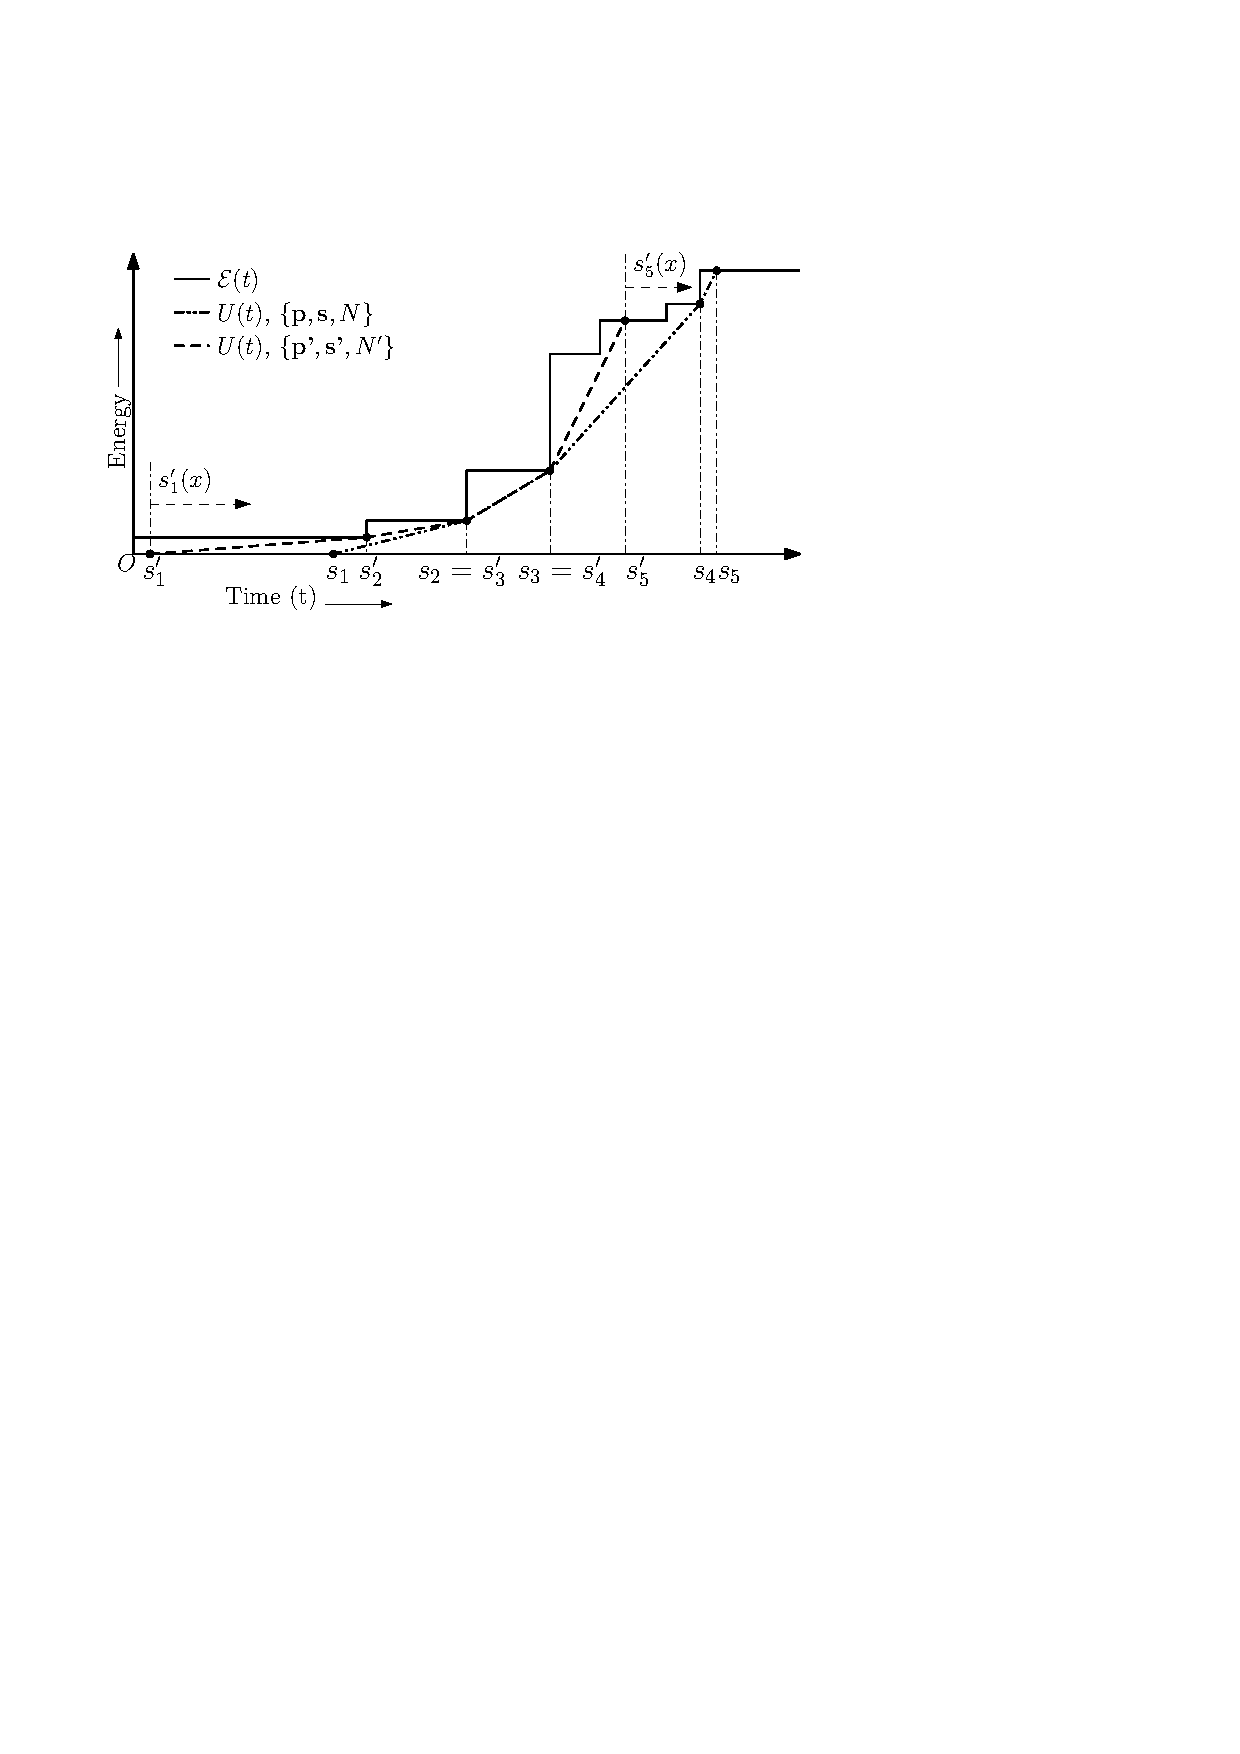
\includegraphics[width=8cm]{Theorem1_sufficient.pdf}}
\caption{Energy curves at Transmitter explaining \textit{Case3} in proof of Theorem \ref{th_algo1_1}}
\label{Theorem1_figure}
\end{figure}

Now, consider the following process which creates child feasible policies from policy $\{\textbf{p'},\textbf{s'},N'\}$ as shown in Figure \ref{Theorem1_figure}. We define two pivots $pv_1$ and $pv_2$. Initially we set $pv_1=s_2'$ and $pv_2=s_{N'}'$. The transmission power right before $pv_1$ is $u$ ($u=p_1'$ initially) and right after $pv_2$ is $v$ ($v=p_{N'}'$ initially). Keeping the policy same from $pv_1$ to $pv_2$ we increase $u$ by a small amount to $u+du$ and decrease $v$ by a small amount to $v-dv$ such that the number of bits transmitted ( i.e. $B_0$) remains same under this transformation. Let $s_1'$ change to $s_1'+x$ and $s_{N'+1}'$ change to $s_{N'+1}'+y$ for some $x,y>0$. We denote such a policy by vectors $\{\textbf{p'(x)},\textbf{s'(x)},N'(x)\}$. Following Lemma \ref{lemma_increase_time}, we can conclude that $(s_{N'(x)+1}'(x)-s_1'(x))<(s_{N'+1}'-s_1')$. We continue increasing $x$ till either $u=p_2$ (in which case we change $pv_1=s_2$) or $v=p_{N'-1}'$ (where we change $pv_2=s_{N'-1}'$) or $s_{N'(x)+1}'(x)$ hits an epoch, say $t_j$ ($pv_2=t_j$, $v\rightarrow\infty$ in this case). After this, we again start increasing $x$ with changed definitions. We continue this process till $x=s_1-s_1'$  or $u$ becomes equal to $v$. Note that the former stopping criteria will be met at a smaller $x$ than the later one since policy $\{\textbf{p'(x)},\textbf{s'(x)},N'(x)\}$ shares at least one epoch with policy $\{\textbf{p},\textbf{s},N\}$ by arguments of previous paragraph. By maintaining these rules we ensure that policy $\{\textbf{p'(x)},\textbf{s'(x)},N'(x)\}$ abides by Lemma 1-5 and is feasible with energy constraint. Since $\left( s_{N'(x)+1}'(x)-s_1'(x)\right)$ is decreasing with $x$, the policy is also feasible with time constraint. As this is continuous on $x$, at $x=s_1-s_1'$ we reach a policy such that $s_1'(x)=s_1$. For $x=s_1-s_1'$, if $s_{N'(x)+1}'(x)\ge s_{N+1}$ then $s_{N'+1}'-s_1'>s_{N'(x)+1}'(x)-s_1'(x)\ge \TRx_0$ and policy $\{\textbf{p'},\textbf{s'},N'\}$ is infeasible with time constraint. If $s_{N'(x)+1}'(x)< s_{N+1}$ then we can follow the arguments in \textit{Case2} to show that policy $\{\textbf{p'(x)},\textbf{s'(x)},N'(x)\}$ is infeasible, which in turn accounts for the infeasibility of policy $\{\textbf{p'},\textbf{s'},N'\}$.
\end{proof}

























%input{Rushil}
\begin{theorem}
The transmission policy, which results from the Algorithm \ref{Algorithm1}, is an optimal solution to Problem 1.
\label{th_algo1_2}
\end{theorem}


\begin{proof}
To prove that the policy (say $\{\textbf{p},\textbf{s},N\}$) described by Algorithm \ref{Algorithm1} is optimal, it is sufficient to show that it abides by the structure presented in Theorem \ref{th_algo1_1}.

To begin with, we prove that the power allocations in Algorithm \ref{Algorithm1} are increasing. We prove this by induction. The base case constitutes of showing that, the initial feasible solution has increasing powers. If INIT\_POLICY returns the constant power policy from time $R$ to $S$ with power $p_c=\frac{\ETx(t_n)}{S-R}=\frac{\ETx(t_n)-\ETx(t_q^-)}{S-t_q}$, then we are done. 

Suppose INIT\_POLICY solves Algorithm 1 from \cite{Yang} with $\widetilde{B}$ bits to transmit after time $t_q$, then the transmission power after time $t_q$ is always increasing. Now, we need to prove that transmission power $p_c$ between time $S$ and $t_q$ is less than the transmission power just after time $t_q$(say $p_i$). Let transmission with $p_i$ end at epoch $t_i$. We prove it by contradiction. Assume that $p_i<p_c$. Following two cases arise.

\textit{Case1:} If $t_i<S$, energy consumed by $p_c$ between time $t_q$ to $t_i$ is 
\begin{align}
&p_c(t_i-t_q)>p_i(t_i-t_q)=(\ETx(t_i^-)-\ETx(t_q^-))\label{eq_1_algo1_modified}
\end{align}
Since $p_c$ uses all energy by $t_q$, the maximum amount of energy available for transmission between $t_q$ and $t_i$ is $(\ETx(t_i^-)-\ETx(t_q^-))$. But by \eqref{eq_1_algo1_modified}, $p_c$ is infeasible between time $t_q$ and $t_i$. As transmitting with $p_c$ was always feasible between $t_q$ and $S$ (and therefore between $t_q$ and $t_i$) in constant power policy, we reach a contradiction.        

\textit{Case2:} If $t_i>S$, then $\ETx(t_i^-)>\ETx(S)=\ETx(t_n)$. So, 
\begin{align}
g(p_i)(t_i-t_q)&=g\left(\frac{\ETx(t_i^-)-\ETx(t_q^-)}{t_i-t_q}\right)(t_i-t_q)
\\
&>g\left(\frac{\ETx(t_n)-\ETx(t_q^-)}{t_i-t_q}\right)(t_i-t_q)
\\
&>g\left(\frac{\ETx(t_n)-\ETx(t_q^-)}{S-t_q}\right)(S-t_q)\label{eq_2_algo1_modified}
\\
&=g(p_c)(S-t_q)=\widetilde{B}.
\end{align}
where \eqref{eq_2_algo1_modified} follows from Property P4. So transmission with $p_i$ from $t_q$ to $t_i$ departs more than $\widetilde{B}$ bits. This is inconsistent with the assumption that the solution we get from Algorithm 1 in \cite{Yang} exactly transmits $\widetilde{B}$ bits after $t_q$. 

Having proved the base case, assume that transmission powers from Algorithm \ref{Algorithm1} are increasing in its $n^{th}$ iteration. The transmission powers between $t_l$ and $t_r$ remain same over iteration $n^{th}$ to $(n+1)^{th}$ iteration, as illustrated in Fig. \ref{figure_Algorithm1}. So, we only need to prove that the transmission power before time $t_l$ is less than the transmission power after $t_l$ and the same for time $t_r$. In $(n+1)^{th}$ iteration, by the definition of the algorithm either $t_l$ updates or $t_{r}$ updates. Assume $t_l$ gets updated to $t_{l}'$, $p_l$ to $p_l'$, $p_r$ to $p_r'$ and $t_r$ remains same. The proof for $t_r$ getting updated can be done with similar arguments and hence we only show proof of this case. If we show that $p_l<p_l'$ and $p_r>p_r'$, then we are done by induction hypotheses. If $t_l$ updates and $t_r$ remains same, then we are certain that $p_{r}'>p_r$ by algorithm definition. Now, from $n^{th}$ step to $(n+1)^{th}$ step, the number of bits transmitted after $t_r$ should decrease as $p_{r}'>p_r$. So, the number of bits transmitted before $t_l$ must be increasing from $n^{th}$ to $(n+1)^{th}$ iteration. This implies that $p_l'$ must also be less than $p_l$. Hence we have proved that the transmission powers are always increasing in the policy being output by Algorithm \ref{Algorithm1}.

Now, we show that transmission powers follow structure \eqref{claim3}. Assume it does not. Specifically, say $p_1$ does not follow structure \eqref{claim3}. The proof for $p_2,p_3..$ can be done likewise. So, $p_1$ has to be more than the minimum possible power i.e. $p_1>\mathcal{P}(s_1,\tilde{s})$, where $\tilde{s}=\argmin_{t_i: s_n < t_i \le s_{N+1}} \mathcal{P}(t_i,s_n)$. Then the amount of energy used by $p_1,p_2,..$ till epoch $\tilde{s}$ can be lower bounded by $p_1(\tilde{s}-s_1)$, as $p_1>p_2..$. But the maximum power available till time $\tilde{s}$ is $\ETx(\tilde{s})=\mathcal{P}(s_1,\tilde{s})(\tilde{s}-s_1)>p_1(\tilde{s}-s_1)$, which is more than what is spent by $p_1$. Hence we reach a contradiction and therefore $p_1=\mathcal{P}(s_1,\tilde{s})$.

Next, we show that Algorithm \ref{Algorithm1} always converges to a policy. From $p_l'<p_l$ and $p_r'>p_r$, we can also conclude that $T_{start}$ and $T_{stop}$ always decrease across the iterations. In all the cases of Algorithm \ref{Algorithm1}, described in Fig. \ref{figure_Algorithm1} (a) (b) (d), we can show, using Lemma \ref{lemma_increase_time}, that $T_{start}-T_{stop}$ always decreases across the iterations. The initial policy to Algorithm \ref{Algorithm1} is given by Algorithm \ref{init_policy}. If the policy output by Algorithm \ref{init_policy}, is the constant power policy returned in line \ref{init_policy_CP}, then initially $T_{start}-T_{stop}=R-S=\widetilde{T}$, where $\widetilde{T}$ is defined in line \ref{init_policy_CP_time}. From line \ref{init_policy_Etn} and \ref{init_policy_CP_time}, 
\begin{align}
& \widetilde{T}g\left(\dfrac{\ETx(t_n)}{\widetilde{T}}\right) = B_0, \TRx_0g\left(\dfrac{\ETx(t_n)}{\TRx_0}\right) \ge B_0
\end{align}    
So $\widetilde{T}\le \TRx_0$ by Property P4. Hence $T_{start}-T_{stop}$ is initially less or equal than $\TRx_0$.

If Algorithm \ref{init_policy} returns policy form line \ref{init_policy_Yang}, then by the properties satisfied by policy presented in \cite{Yang}, we know that the transmission powers would be increasing after time $t_q$. This policy is same as policy in line \ref{init_policy_CP} till time $t_q$. As transmission with power $p_c$ after $t_q$ finishes transmission of $B_0$ bits till time $S$, the policy form line \ref{init_policy_Yang}, transmitting with atleast $p_c$ or more power after $t_q$, would definitely finish before time $S$. So $T_{start}-T_{stop}$ in the initial iteration of Algorithm \ref{Algorithm1} must be less than or equal to $(R-S)=\TRx_0$.

%As $T_{stop}$ decreases in every iteration of the algorithm, $t_r$ must also decrease globally, though it can increase in few iterations. Hence we can be sure that $t_r$ can potentially reach $t_q$ (Initially $t_r>t_q$). If it does reach $t_q$, then the policy    
 
We are sure that Algorithm \ref{Algorithm1} always converges to a solution which satisfies structure \eqref{claim2} and \eqref{claim4}, by the arguments presented before Theorem \ref{th_algo1_1}. Hence, all structures are satisfied and the Algorithm results in an optimal solution.

%      
% 
%First we prove that the power allocations in Algorithm \ref{Algorithm1} are in accordance with \eqref{claim3}. In any particular iteration of the algorithm, we select the maximum transmission power between $t_{l}$ and all epochs before lying in range $t_{start}$ to $t_l$. Let $t_j$ be the epoch which amounts to the maximum power and $p_j$ be the maximum power, i.e. 
%\begin{align}
%&t_j=\argmax_{t_i:t_{start}\le t_i< t_l} \max\left(\frac{\ETx(t_l^-)-\ETx(t_i^-)}{t_l-t_i}, \frac{\ETx(t_l^-)}{t_l-t_{start}}\right)
%\\
%&p_j= \max_{t_i:t_{start}\le t_i< t_l} \max\left(\frac{\ETx(t_l^-)-\ETx(t_i^-)}{t_l-t_i}, \frac{\ETx(t_l^-)}{t_l-t_{start}}\right)
%\label{eq_max_algo1_2}
%\end{align}
%We claim that this is indeed the maximum over all $t_i$'s in range $s_1$ to $t_l$. To prove this by contradiction, assume that $\exists t_{a}: s_1\le t_{a}<t_{start}$ and $p_{a}=\dfrac{\ETx(t_l^-)-\ETx(t_a^-)}{t_l-t_a}>p_j $. From \eqref{eq_max_algo1_2}, we can say that 
%\begin{align}
%&\ETx(t_l^-)\le p_j(t_l-t_{start}),\\
%&\implies \ETx(t_l^-)<p_a(t_l-t_{start}).
%\end{align}
%But transmission with power $p_a$ consumes $p_a(t_l-t_{start})$ amount of energy between $t_j$ and $t_l$, which is more than the maximum available energy till $t_l$ i.e. $\ETx(t_l^-)$. Hence transmission with $p_a$ is infeasible. 
%
% 
%Now we seek to show that this procedure of selecting maximum slopes going 'backwards' also gives us the minimum slopes going 'forwards', as described in \eqref{claim3}.\\
%We shall show this by contradiction. Let $t_i$, $t_j$ and $t_k$ be three consecutive corner points where the power of transmission increases, as per our allocation. Now suppose, it is possible to transmit with a lower power between $t_i$ and some $t'_j$. 
%Then the power of transmission between $t_j$ and $t_k$ is not the maximum power since we could transmit at a higher power from $t'_j$ and $t_k$. Which is a contradiction as this is not consistent with out allocation algorithm.\\
%Therefore, the allocation policy before point $t_q$ is consistent with the structure.. (See figure)
%We can prove similarly for the powers after point $t_q$.
\end{proof}




